\section{Introduction}
The integration of robots is rapidly expanding across various domains, spanning from industrial automation to healthcare, agriculture, and domestic services. The ability to manipulate objects is fundamental for robots to perform a variety of tasks in these diverse domains \cite{technologies9010008, doi:10.1146/annurev-control-060117-104848}. Among the different categories of objects that robots encounter, liquids present a unique challenge due to their complex behavior. Despite the importance of robotic fluid manipulation in various applications such as handling hazardous materials in laboratories to facilitating assistive feeding technologies designed for differently-abled individuals, research in robotic fluid manipulation is under-explored and challenging for several reasons.
\begin{figure}
    \centering
    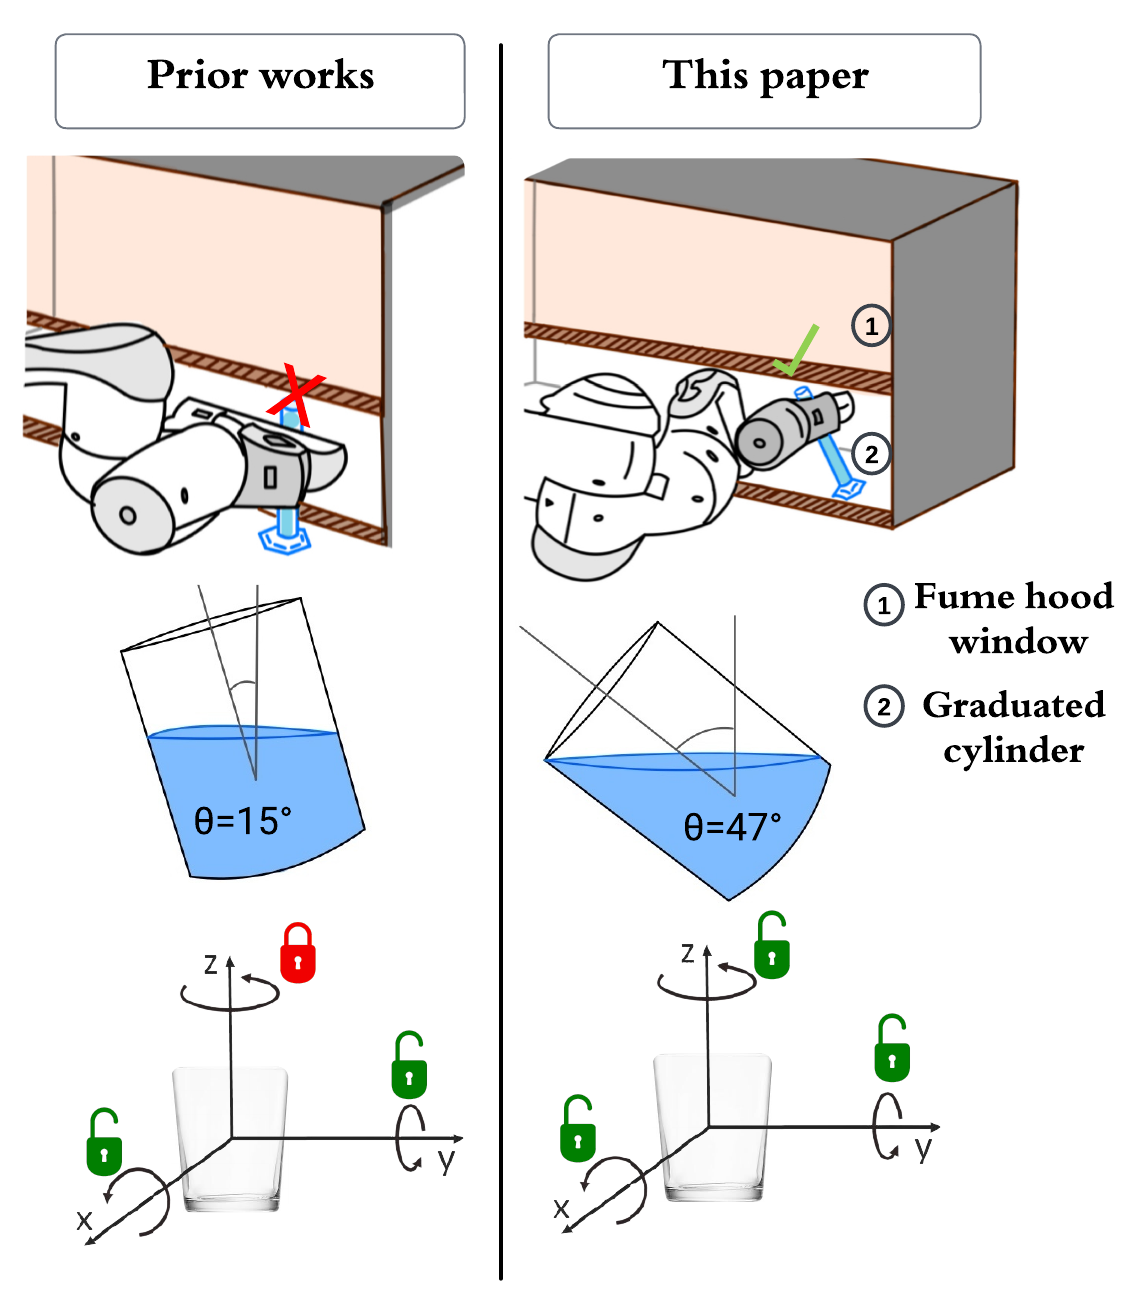
\includegraphics[width=\columnwidth]{figs/camera_ready_first_page_figure.png}
    \caption{
    Motivated by the need for robots to perform in cluttered environments such as a chemistry setup where robots must transport chemistry vessels inside a fume hood (\textsl{top row}), 
    this paper targets the challenge of enabling spill-free liquid transport while avoiding obstacles. Our approach introduces two key enhancements over existing methods: (i) increasing the allowable tilt angle to the maximum quasi-static spill-free tilt angle, rather than the limited angles used previously \cite{pendulum, pendulum2019} (\textsl{second row}); (ii) enabling rotation about all axes throughout the trajectory, instead of maintaining fixed yaw or orientation (\textsl{third row}) \cite{pendulum,  springdamper2021}.
    }
    \label{fig:first_page_figure}
    % \vspace{-15pt}
\end{figure}


Fluid manipulation is challenging due to the intricate and nonlinear nature of fluid dynamics. Accurately modeling fluid dynamics is heavily task-dependent and requires substantial computational resources, hindering real-time control \cite{systemstudy1, systemstudy2}. Existing approaches tackle these challenges by simplifying the complex fluid dynamics into more computationally efficient linearized pendulum or mass-spring-damper models. However, these methods struggle in cluttered scenes due to several reasons. These linearized models restrict the motions to pendulum-like or mass-spring-damper-like behavior \cite{pendulum2, pendulum2018, pendulum, springdamper2022, springdamper2021, pendulum2019}. Additionally, these approaches impose restrictions on the container's orientation by setting fixed or limited Euler angle ranges throughout the trajectory \cite{pendulum, springdamper2021}. Moreover, these methods rely on constant monitoring of the liquid surface to execute trajectories, which can be obstructed by opaque fumes produced by the liquid or by obstacles present in cluttered scenes \cite{spill1, pendulum2019,montazeri2013chemical}. Consequently, the action space is over-constrained, and the robot can only perform limited motions, inhibiting its ability to maneuver around obstacles in cluttered environments.


To address these limitations, we propose Spill-Free RRT* (\textit{SFRRT*})\footnote{Open-source code and video at: \href{https://avv-va.github.io/sfrrt}{https://avv-va.github.io/sfrrt}.}, for spill-free manipulation of open-top liquid-filled containers, particularly in cluttered environments. Our method enables these advantages (\cref{fig:first_page_figure}):
(i) \textsl{Increased action space}, so that the robot can operate effectively in cluttered scenarios. We do this by training a model to implicitly learn liquid dynamics to capture the correlation between container trajectory and spillage risk, 
(ii) \textsl{No additional information needed}. Our method relies solely on the robot and the container shape to operate and does not require constant monitoring of the liquid surface. 


To achieve this, SFRRT* generates spill-free trajectories through these key contributions: (i) it first uses the container shape to inform the generation of a spill-free path via RRT*. By considering the container geometry, the algorithm calculates the maximum tilt angle beyond which the container will spill and constrains the path search accordingly (\cref{subsec:informed-geometric-path-planner}). (ii) Subsequently, our method generates a spill-free trajectory from this path by using a time-parameterization algorithm in conjunction with a transformer-based neural network classifier. The neural network, trained on a dataset of container trajectories, predicts whether a given trajectory is spill-free or not, allowing SFRRT* to set the trajectory's jerk to avoid spills (\cref{method:timepar}), (iii) Lastly, to train the transformer-based neural network, we produce a dataset of 700 container trajectories collected from individuals handling different container scenarios.



% State-of-the-art approaches for robotic fluid manipulation struggle in cluttered environments due to simplified liquid models,
% and challenging due to several reasons
% Robotic fluid manipulation plays a crucial role in various applications, ranging from handling hazardous materials in laboratories to facilitating assistive feeding technologies designed for differently-abled individuals. Despite its importance, research in this field remains underexplored due to several reasons. 
% \ava{Robots are increasingly integrated into critical applica-
% tions, ranging from industrial automation to healthcare and
% even space exploratio}
% ava{there has been research in rigid and soft bofy manipulation but fluid manipulation remains underexplored and challenging for sevelar reasons. }
% \ava{depending on the fluid it coud be hazardous}
% Robots are increasingly integrated into critical applications, ranging from industrial automation to healthcare, agriculture, and domestic service. Robotic manipulation is an essential skill for robots to perform a variety of tasks in these domains. Among the different types of objects that robots may encounter, fluids pose a unique challenge due to their complex and dynamic behavior. Robotic fluid manipulation has applications ranging from hazardous materials in laboratories to facilitating assistive feeding technologies designed for differently-abled individuals \cite{chem1, chem2, assistfeed1, assistfeed2}. However, research in robotic fluid manipulation remains underexplored and is challenging for several reasons.
% Robots are increasingly integrated into critical applications, ranging from industrial automation to healthcare. 
% Fluid manipulation is a ubiquitous task across both industrial and domestic settings. It plays a pivotal role in critical applications ranging from managing hazardous materials in laboratories to facilitating assistive feeding technologies designed for differently-abled individuals \cite{chem1, chem2, assistfeed1, assistfeed2}. 
% There has been research in rigid and soft body manipulation but fluid manipulation remains underexplored and is challenging for several reasons.
% It plays a pivotal role in critical applications ranging from managing hazardous materials in laboratories to facilitating assistive feeding technologies designed for differently-abled individuals \cite{chem1, chem2, assistfeed1, assistfeed2}
% Fluid manipulation is a ubiquitous task across both industrial and domestic settings. It plays a pivotal role in critical applications ranging from managing hazardous materials in laboratories to facilitating assistive feeding technologies designed for differently-abled individuals \cite{chem1, chem2, assistfeed1, assistfeed2}. 
% Robots have the potential to empower these applications, however, robotic fluid manipulation is challenging for several reasons.




% (iii) \textsl{Computational efficiency}:  SFRRT* is a sampling-based approach and takes less than 30 seconds to generate spill-free trajectories.


% R1ather, it leverages container geometry to effectively explore the spill-free space and  then it utilizes
% demonstratid container trajecories 
% the container trajectruy tp set the fourth order postiiotn derivaties (jerk) to generate spill-free trajectories. By doing this we aim to enable these advantages:

% Overall, this work enables spill-free manipulation of liquids in cluttered environments without requiring monitoring of the liquid surface. 
% By employing a machine-learning model inherently nonlinear to capture the correlation between container trajectory and spillage risk,


% Rather, 
% Rather, it captures liquid dynamics intrinsictly through demonstarted container trajectories
% For instance, considering two containers holding equal amounts of liquid, the one with a larger volume can be tilted to higher angles without causing spills. Moreover, it can sustain higher velocities without risking spills. Thus, by modeling the relationship between the container and spillage risk, and using that to control the container's trajectory, SFRRT* generates spill-free trajectories.

% Insteadof modeling the luqyud, we train a transformer based model that implictklu captures 



% Fluid manipulation is a ubiquitous task across both industrial and domestic settings. It plays a pivotal role in critical applications ranging from managing hazardous materials in laboratories to facilitating assistive feeding technologies designed for differently-abled individuals \cite{chem1, chem2, assistfeed1, assistfeed2}. Robots have the potential to empower these applications, however, robotic fluid manipulation is challenging.

% Overall, this work enables spill-free manipulation of liquids in cluttered environments without requiring constant monitoring of the liquid. Our key advantages include: (i) \textsl{increased reachable space}:  
% By using a machine-learning model (that is inherently nonlinear) to capture the relationship between the container trajectory and spillage risk, instead of enforcing a linearized liquid model, the robot can execute more flexible and diverse trajectories and as a result can perform in cluttered scenarios, (ii) \textsl{no additional information needed} unlike existing approaches that rely on an external sensor to continuously monitor the liquid surface which could get obstructed in cluttered scenarios, this method requires no external information (iii) \textsl{computational efficiency}: in contrast to approaches that use computational fluid dynamics which is computationally expensive, this is a sampling-based approach and takes less than 30 seconds to generate a spill-free trajectory.


% Overall, this work enables spill-free manipulation of liquids in cluttered environments without requiring constant monitoring of the liquid. Key contributions of this work include:
% \begin{enumerate*}[label=(\roman*)]
%   \item a transformer-based neural network designed for classifying trajectories as either spill-free or not(\cref{method:timepar}),
%   \item an informed sampler formalized based on container shape to guide spill-free space exploration (\cref{subsec:informed-geometric-path-planner}) and,
%   \item 700 container trajectories collected from individuals handling different container scenarios that are used to train the model.
% \end{enumerate*}

% This framework provides the following advantages for enabling spill-free fluid manipulation: 1) \textsl{Kinematic Flexibility}: in deviation from pendulum-based models that impose restrictive kinematic constraints (see \cref{subsec:comparison}), our approach is unencumbered by such limitations; 2) \textsl{Computational Efficiency}: in contrast to CFD-based approaches that necessitate extended computational times, our planner is capable of generating spill-free trajectories in less than $30$ seconds, as detailed in \cref{subsec:eval-spill-rate}); and, 3) \textsl{Focus on Spill-Free, not Slosh-Free}: while prior work primarily addresses slosh-free or constrained-slosh trajectories \cite{spill1, spill2, spill3}), our model specifically aims to prevent spills---a capability that should cover a larger number of practical scenarios. While there are a few approaches that focus on spill-suppression, they either use CFD which is costly \cite{meal1}, or they need to model the slosh dynamics in every step of the trajectory using an external sensor \cite{slosh1}.

% The central challenge in robotic fluid manipulation is the real-time prediction and control of fluid dynamics. This work focuses on enabling robots to manipulate open-top liquid-filled containers without spilling in cluttered scenarios, a cornerstone in automated fluid-handling tasks. Liquid manipulation is challenging due to fluid dynamics' intricate and nonlinear nature. Moreover, accurately modeling fluid dynamics is heavily task-dependent and requires substantial computational resources, hindering real-time control \cite{systemstudy1, systemstudy2}.

% Existing approaches tackle these challenges by simplifying the complex fluid dynamics into more computationally efficient linearized pendulum or mass-spring-damper models. However, these methods struggle in cluttered scenes. This is because these models generate trajectories that are restricted to following pendulum- or mass-spring-damper-like motions. Moreover, they impose kinematic constraints such as restricting trajectories to two dimensions or fixed end-effector orientations. These approaches also require constant visual monitoring of the liquid which could get obstructed in cluttered scenes \cite{pendulum, springdamper2022, spill1}.

% In contrast, this work takes a fundamentally different approach that removes the need to explicitly model the liquid itself. Instead, we focus solely on leveraging the motion and shape of the container to generate spill-free trajectories. By doing so, we eliminate the constraints imposed by simplified liquid models, enabling the robot to maneuver flexibly in cluttered environments. This necessitates modeling the relationship between the container's trajectory and spillage risk.

% To build an understanding of this relationship, we recorded individuals transporting containers of liquid, using motion capture to track the containers' trajectories. We then classify whether each trajectory caused a spill or not. From this dataset composed of real-world demonstrations, a transformer-based (\cite{transformers}) machine learning model was trained to categorize containers' trajectories as spill-free or not. This model implicitly captures the nonlinear fluid behaviors. We call this model the Spill-Free Classifier (SFC) which is later utilized to generate a spill-free trajectory.
% To generate a spill-free trajectory, we first leverage the container's shape to guide RRT* in generating a collision-free path. Using the container's shape to inform the RRT*, allows for avoiding states such as the container being upside down or tilted beyond its capacity. Then, leveraging the SFC, we parameterize the path, such that the SFC predicts the resulting trajectory is spill-free. 

% SFC's nonlinear nature expands the robot's reachable space by removing constraints seen in simplified liquid models, such as restricting the trajectory to follow a pendulum-like trajectory. It also doesn't impose kinematic constraints such as fixed orientations. Instead, it uses the container's shape to inform the path, which allows the container to be tilted as long it doesn't spill.
% Overall, this work enables spill-free manipulation of liquids in cluttered environments without requiring constant monitoring of the liquid. Key contributions of this work include:
% \begin{enumerate*}[label=(\roman*)]
%   \item a transformer-based neural network designed for classifying trajectories as either spill-free or not(\cref{method:timepar}),
%   \item an informed sampler formalized based on container shape to guide spill-free space exploration (\cref{subsec:informed-geometric-path-planner}) and,
%   \item 700 container trajectories collected from individuals handling different container scenarios.
% \end{enumerate*}



% \ar{from now on it gets confusing, it's not clear what is a contribution and what is introduction. This is how it reads:}\\
% \ar{this paper has this goal}\\
% \ar{we use transformers. This is because of blablabla}\\
% \ar{we have a novel two step process. we call it SFRRT*. Wait what? I thought you just used transformers}\\
% \ar{it is composed of two steps. Wait What? where is the transformer coming from then?Is it part of the contribution? Is it the same as the second step? Dunno}
% \ar{then you just say that the only novelty is transformers}


% This paper targets the specific challenge of spill-free manipulation of open-top liquid-filled containers in obstacle-rich settings by introducing a novel framework for the modeling and planning of such robot motions. 

% Departing from conventional, simplified slosh models, we propose a transformer-based machine-learning approach that captures the nonlinear dynamics of liquid spillage \cite{transformers, alphastarblog, protein}. Central to this approach is the elimination of reliance on external sensors for spillage prediction, since our model utilizes the robot's internal sensing capabilities, predicting spillage based on the container's movements alone. 
% Additionally, this method enables our system to navigate complex environments using the robot's full range of motion, without imposing constraints on the robot's degrees of freedom or the container's shape.
% The inherent nonlinearity of our learned model allows for adaptable and precise spillage prediction, thereby making it applicable to a variety of container shapes and scenarios. 
% The generation of spill-free trajectories is accomplished efficiently, typically in less than a minute, through a novel two-step planning process that we term \textsl{Spill-Free RRT*} (\textsl{SFRRT*}).

% The first step of \textsl{SFRRT*} involves a sampling-based planner with an informed sampler, designed to account for the specific properties of various containers. This planner produces waypoints that are later assembled into a spill-free trajectory.
% The second step involves parameterizing these waypoints, using a transformer-based neural network to classify these trajectories based on their spill-free properties. This model determines the maximum speed for traversing the waypoints while ensuring spill-free conditions.
% Our two-step approach not only ensures spill-free trajectories but also enhances the system's modularity, which allows for the integration of diverse planners and time parameterization approaches, accommodating different requirements.

% To our knowledge, SFRRT* is the first framework to employ a transformer-based architecture to generate spill-free trajectories. Overall, this work contributes: 
% \begin{enumerate*}[label=(\roman*)]
%   % \item a novel modular framework to generate spill-free trajectories that overcome the shortcomings of previous works (\cref{fig:system_diagram}),
%   \item a transformer-based neural network designed for classifying trajectories as either spill-free or not (\cref{method:timepar}), and
%   \item an informed sampler formalized based on container properties to sample spill-free states (\cref{subsec:informed-geometric-path-planner})
%   \item 700 trajectories collected from multiple individuals handling different container scenarios.
% \end{enumerate*}